
\documentclass[conference]{IEEEtran}
\renewcommand\thesection{\Alph{section}}
\usepackage{graphics}
\usepackage{framed,graphicx}
\newcommand{\tion}[1]{\ref{sect:#1}}
\newcommand{\eq}[1]{Equation~\ref{eq:#1}}
\newcommand{\fig}[1]{Figure~\ref{fig:#1}}
\newcommand{\bi}{\begin{itemize}}
\newcommand{\ei}{\end{itemize}}
\newcommand{\be}{\begin{enumerate}}
\newcommand{\ee}{\end{enumerate}}

\begin{document}
\pagestyle{plain}
\noindent
\textbf{Responses to reviewers\\}

\noindent
\textit{A. Reviewer 1}

\textit{Topic modeling has been used in many software engineering papers. The paper shows that topic modeling, especially LDA, suffers from order effects -- which is new and interesting. Depending on the order data is presented to LDA, it produces a different model. Search-based software engineering can be used to tune LDA parameters so that order effect is minimized. LDADE (LDA mixed with Differential Evolution) is presented. It is shown to improve standard LDA for various settings including classification of StackExchange websites into relevant and non-relevant documents -- which is good.}

Thank you for those kind words.

\noindent
\textit{\\A.1.}
\textit{Very closely related work exists:}

\textit{A prior work has demonstrated suboptimal performance of topic modeling, in particular LDA, when default parameters are used, and proposed a solution that addresses the problem using search-based software engineering~\cite{panichella2013effectively}. Thus, the novelty of the work seems limited. The paper does not describe why LDADE is better than Panichella et al.'s work. Panichella et al.'s work (LDA-GA) should have been prominently highlighted in the introduction of the paper and a short discussion should be given as to why another search-based solution is needed.\\}

We have updated the introduction section to highlight the difference between LDA-GA and LDADE. We have also compared the results of LDADE against LDA-GA in section 5.8.
Panichella et al. didn't consider the problem of order effects. Their method of using Genetic Algorithm to find optimal configurations is time extensive task. We ran LDA-GA and compared our stability ($\Re_n$) delta score against LDADE. We observed that LDADE is much faster and gets much stable results. 


\noindent
\textit{\\A.2.} 

\textit{The experiments need to be improved in the following ways/ First, LDA has been used to help many realistic software engineering tasks (for example, tasks considered by papers included in Table 2. There is a need to expand the experiments to compare LDA and LDADE on those realistic software engineering tasks. It is unclear if the task considered in the experiments (Section 5.3) is realistic (why categorizing StackExchange data into relevant and non relevant categories useful?). More than one tasks should have been considered (similar like Panichella et al.'s work).\\}

Firstly, we found out that about 24 out of 28 papers referenced in Table 2 uses unsupervised LDA for further analysis. This shows that there is a heavy need for LDA in unsupervised tasks. Secondly, we first thought to reproduce Panichella et al. results, but the link provided in the paper is not available anymore. So we couldn't validate their results. We didn't have access to any other open source datasets which were about those realistic software engineering tasks. Since all the SE tasks can be categorized into unsupervised and supervised problems, our results show an improved performance for both kinds of problems. One could argue that performances of LDA should be accessible before applying it to a specific task. This measure should be independent from the supported SE task. And that's the reason, we have used Jaccard similarity which gives an internal measure of how good cluster quality is.

\noindent
\textit{\\A.3.} 

\textit{Second, there is a need to compare Panichella's work (LDAGA) with LDADE on some realistic software engineering tasks. It is unclear if LDADE is better than LDAGA.\\}

See A.1.

\noindent
\textit{\\A.4.}

\textit{The results reported in Section 5.3 are questionable. Why not use LDADE to tune all 3 parameters of LDA (k, alpha, beta)? f k is fixed and alpha and beta are fixed too, what parameter(s) is tuned then?\\}

 Sorry, that was our mistake in the text. We did not tune separately. We tuned for all 3 at once. We have corrected the text to make that clearer. See Section 5.3.

\noindent
\textit{\\A.5.}  

\textit{Why untuned (with $k = 10$) is compared with tuned (with k = 20, 40, 80, and 200)? Shouldn't they be compared under the same setting of $k$? \\}

You are right that the comparison should be done under the same setting of $k$. But most libraries provide the default parameter as $k=10$. And researchers are left with the challenge of the proper selection of configurations. The researchers finally use some heuristics to come up with the value of $k$ for their analysis. But we can see that for some datasets $k=80$ matters and for some $k=200$. And LDADE finds this kind of settings automatically. And this also holds true with the original Blei study~\cite{blei2003latent} that, for the classification task value of $k$ matters the most.

\noindent
\textit{\\A.6.} 

\textit{Is k-fold cross validation used?  Is training data kept separate from test data (including during the tuning phase)? \\}

Yes, 5-fold stratified cross validation was used. 80\% was used as training and 20\% as testing, and for the tuning phase, out of 80\%, 65\% was used for training and 15\% as validation set.

\noindent
\textit{\\A.7.}  

\textit{Why F2 rather than F1 or F1/2? Is the difference statistically significant? \\}

 We did F1 and F2 analysis both, and in both the cases LDADE selected the optimal configuration and performed better. But since we were working with industrial partners on the classification task, they wanted F2. This is the reason why we showed F2 results. In Figure~\ref{fig:f1}, we show LDADE is improving the F1 results as well. We have updated the Figure 8 with variance which is inter-quartile (75th-25th percentile) range. We can see how stable our results are, and the improved performance of tuned over untuned is statistically significant.

\begin{figure}[!htbp]
  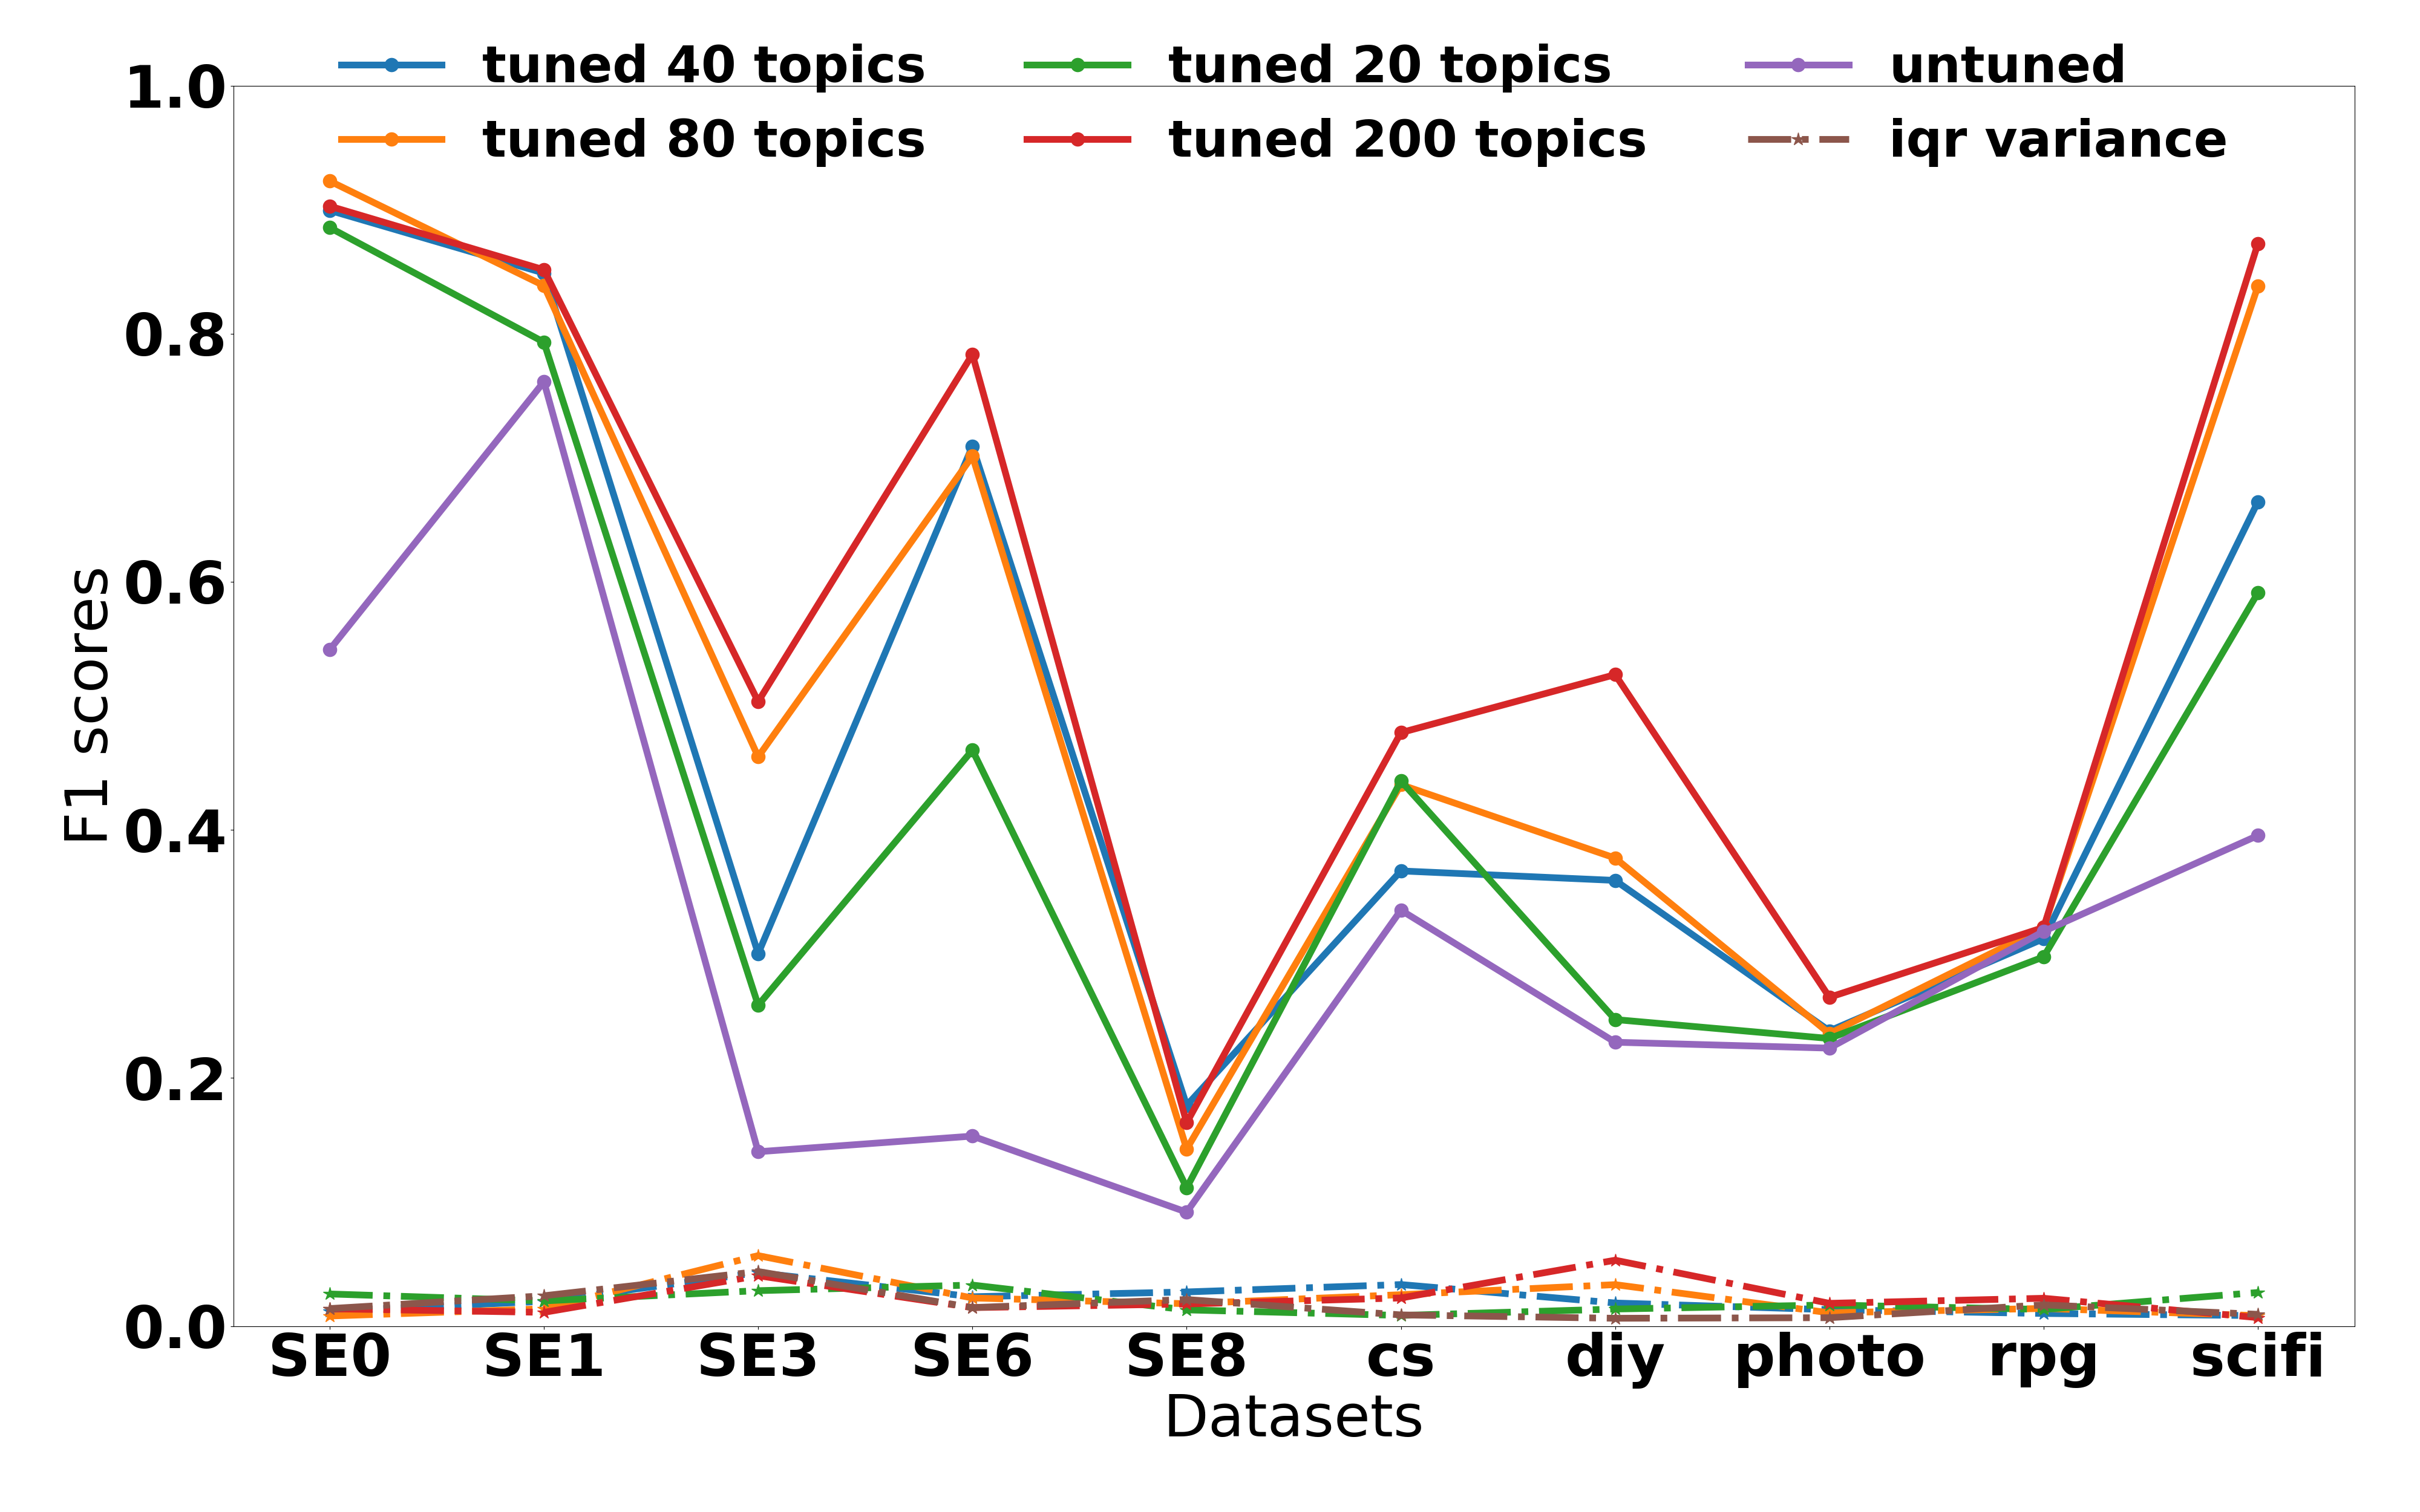
\includegraphics[width=\linewidth]{./fig/F1.png}
  \caption{Tuning and Untuned results for Classification SE Task}
  \label{fig:f1}
\end{figure}

\noindent
\textit{\\A.8.}  

\textit{Minor issues:}
\textit{
\bi
\item Why need to evaluate across different platforms (Linux, Macintosh)? Wouldn't the platform be irrelevant?
\item Related work is revised $->$ is reviewed
\item S2 $->$ Section 2 (similarly for S1, S3, and so on)
\item The period of time considered for drawing Table 1 needs to be mentioned. 
\item Should Table headings be at the top of tables? Need to confirm with IST guidelines.
\item Reference 69 is incomplete.\\
\ei}

That is our mistake in text, we wanted to say that we performed the experiments on any kind of Linux platform. Thank you for other suggestions. We have fixed them.

\noindent
\textit{\\A. Reviewer 2}

\textit{SUMMARY: The authors empirically analyze the instability of LDA and the importance of its parameters' tuning. Then the authors present LDADE, a search-based software engineering tool that tunes LDA parameters using DE (Differential Evolution). An empirical study indicate that by using LDADE, the topic modeling technique is much more stable and reliable.}

\textit{EVALUATION: This is a very interesting paper. It is in general well-written and easy to follow. I really like the goal of the paper. Having worked with LDA I totally agree that using the technique as a ``black-box'' is not recommended. So, the idea of using LDADE to (i) improve the stability of LDA and (ii) reduce the threats that could affect the validity of the results achieved due to an incorrect configuration of the technique is really important. Thus, I think that the paper has a great potential.\\} 

Thank you for those kind words

\noindent
\textit{\\B.1.} 

\textit{The first issue is related to the description of LDADE. I have to admit that Section 4.3 of the paper is quite difficult to follow. First of all, I strongly suggest to the authors to provide a ``bird-eye-view'' of the approach before providing the details. Which is the output of LDADE? How can I use such an output? If I understood correctly, the output of LDADE is just a set of topics (similar to the output of LDA). Is this correct? If so, the authors should explicit mention this. Also, an usage scenario of LDADE could be worthwhile.\\}

We have updated the algorithm in section 4.3 and have provided the bird-eye-view of our approach. Yes, the output of LDADE is just a set of topics but this time these topics will be more stable. For usage, please see A.2. Since so many people have been using unstable LDA, LDADE could provide stability and conclude better results.

\noindent
\textit{\\B.2.}  

\textit{In addition, I did not understand at all when and how LDADE varies the parameters of LDA (k, alpha and beta). LDA in LDADE is invoked through the function ldascore. However, in such a function k, alpha and beta are set to default values.\\}

Sorry about that we did not clear this in the text. Ldascore function is invoked which is same as algorithm 1 but this time rather than having default parameters as input, ldascore takes the tuned parameters generated from DE. We have made this more clearer in section 4.3.

\noindent
\textit{\\B.3.} 

\textit{I appreciated that the authors reported the pseudo-code of LDADE. However, I think that a much deeper description of each step is required. The authors should explain each step of the algorithm and more important should define each function/variable of the pseudo-code. For instance, Data is never instantiated in Algorithm 2 (probably because it is an input?). Or, which is l[0] in Algorithm 1. Another imprecision is related to the function ldascore. From Algorithm 1, ldascore takes as input n and Data. In Algorithm 2 ldascore is called at line 11 passing as parameter Si (a population?) and at line 12 Si, n and Data. Also, Cur\_Gen is used as a matrix. However, when calling on Cur\_Gen the method ``add'', four parameters are passed. I understand that it is just a pseudo-code. However, a much higher level of formality is required.\\}

Thank you for pointing out those. We have provided a better explanation of Algorithm 2 in Section 4.3. 

\noindent
\textit{\\B.4.} 

\textit{I still have some doubts about how DE is used. Specifically, I would like to see much more details on the technique (to make the paper self-contained) and (much important) the design of the approach. For instance, which is the encoding of each solution? Which are the operators used to evolve the solutions? Which is the quality/fitness function? Looking at the pseudo-code, it seems that the quality function is represented by ldascore. If so, why scores are encoded in the solution?\\} 

We have fixed that by providing a better explaining of the Algorithm 2 in section 4.3.

\noindent
\textit{\\B.5.}  

\textit{The authors provide empirical evidence that LDA used with default configuration parameters is not stable. What about if LDA is configured properly - for instance by using LDA-GA? In other words, which are the results achieved if in the algorithm 1 instead of using LDA, the authors try to use LDA-GA?\\}

Please see A.1.

\noindent
\textit{\\B.6.}  

\textit{Could the instability be due to an incorrect configuration of the LDA parameters? This is a critical point that should be addressed in the paper.\\}

Sorry, that is the whole objective of this paper. We need to find correct configuration faster and which makes LDA more stable.

\noindent
\textit{\\B.7.}   

\textit{Turning to the empirical evaluation, the main problem here is related to the lack of a deeper analysis of the results achieved. For instance, looking at Figure 6 it seems that the results achieved on “PitsC” are quite stable. Why? Did the authors have some clues on why on this particular dataset the untuned LDA provides quite acceptable results? Here a qualitative analysis of the results achieved could be worthwhile.\\}

Sorry, I believe you mistook it for PitsD. We are seeing the largest improvements in PitsD, that is because what kind of data it represents. About 92\% of the data samples report the severity of level 3.  All the other Pits Datasets have mixed samples of severity level. This also proves that LDADE gets better cluster when data is not skewed, where as on the other hand even the data is not skewed, LDA was providing bad performance.

\noindent
\textit{\\B.8.} 

\textit{A qualitative analysis could be also useful to better explain why LDADE provides much more benefits on VEM than Gibbs. Note that this result also confirms the results achieved in the literature about the higher stability of Gibbs as compared to other implementation of LDA.\\}

VEM only gets you to a local optimum that depends on initialization and other factors in the optimization problem~\cite{asuncion2009smoothing}. On the other hand a good sampling algorithm like gibbs sampling can achieve the global optimum. In practice because of finite number of samples that are used, sampling can give you a sub-optimal solution. LDADE works as another kind of sampler which selects good priors at the initialization can achieve better sub-optimal solutions and that is the reason why LDADE has better benefits on VEM.

\noindent
\textit{\\B.9.} 

\textit{Very interesting is the analysis of the Delta score. However, in some cases the improvement in terms of stability is not so high. Also here could be worthwhile to discuss in details such cases. In addition, is there any statistical significant difference between the achieved scores? An analysis of the results supported by statistical tests could strengthen the findings.\\}

To explain why stability is achieved better in some cases and not in some cases, please look at our explanation in B.7. And we have also explained whether our results achieved are statistically significant or not in A.7.

\bibliographystyle{elsarticle-num}
\medskip
\bibliography{main}

\end{document}


